\documentclass{article}

\usepackage[letterpaper, portrait, margin=1.5in]{geometry}

\usepackage{fancyhdr}
\usepackage{ragged2e}
\usepackage{graphicx}
\usepackage{caption}
\usepackage{amsmath}
\usepackage{rotating}

\usepackage{listings}
\usepackage{color}

\definecolor{dkgreen}{rgb}{0,0.6,0}
\definecolor{gray}{rgb}{0.5,0.5,0.5}
\definecolor{mauve}{rgb}{0.58,0,0.82}

\lstset{frame=tb,
  language=Java,
  aboveskip=3mm,
  belowskip=3mm,
  showstringspaces=false,
  columns=flexible,
  basicstyle={\small\ttfamily},
  numbers=none,
  numberstyle=\tiny\color{gray},
  keywordstyle=\color{blue},
  commentstyle=\color{dkgreen},
  stringstyle=\color{mauve},
  breaklines=true,
  breakatwhitespace=true,
  tabsize=4
}

\setcounter{secnumdepth}{1}

\usepackage{chngcntr}
\counterwithin{figure}{section}

\renewcommand*{\thepage}{C\arabic{page}}

\pagestyle{fancy}
\lhead{ACME Robotics}
\chead{\#8367}
\rhead{\ifcontents Contents \else Week \thesection \fi}

\newif\ifcontents
\contentstrue

\makeatletter
\renewcommand{\@seccntformat}[1]{}
\makeatother
\begin{document}

\subsection{Increase the Intake arm Length and Thickness}
%! Re-make the intake arms out of thicker material
Ashlin and Aidan realized that another way to increase the speed and effectiveness of the intake was to increase the reach of the third intake roller (the one that flops down into the crater). They decided that if the whips were an inch longer this would significantly increase the reach of the whips while not slowing it down. In order for this to work the roller arm need to be increase an inch in length and positioned an inch higher so that the whips did not hit the ground or crater to much that they might cause unnecessary friction. New arms were cut out however a belt for the new length did not exist. So the team decided to not increase the arm or whip length, but did increase the arm thickness as shown in figure \ref{fig:arm} They did this because they knew from experience that the arms often had to absorb significant impact from collisions and previous arms had snapped because of this. The team believed that increasing the thickness would result in more durability. The new arms were cut and put on the robot, where they were tested and found to be very strong and durable.

\begin{figure}
    \centering
    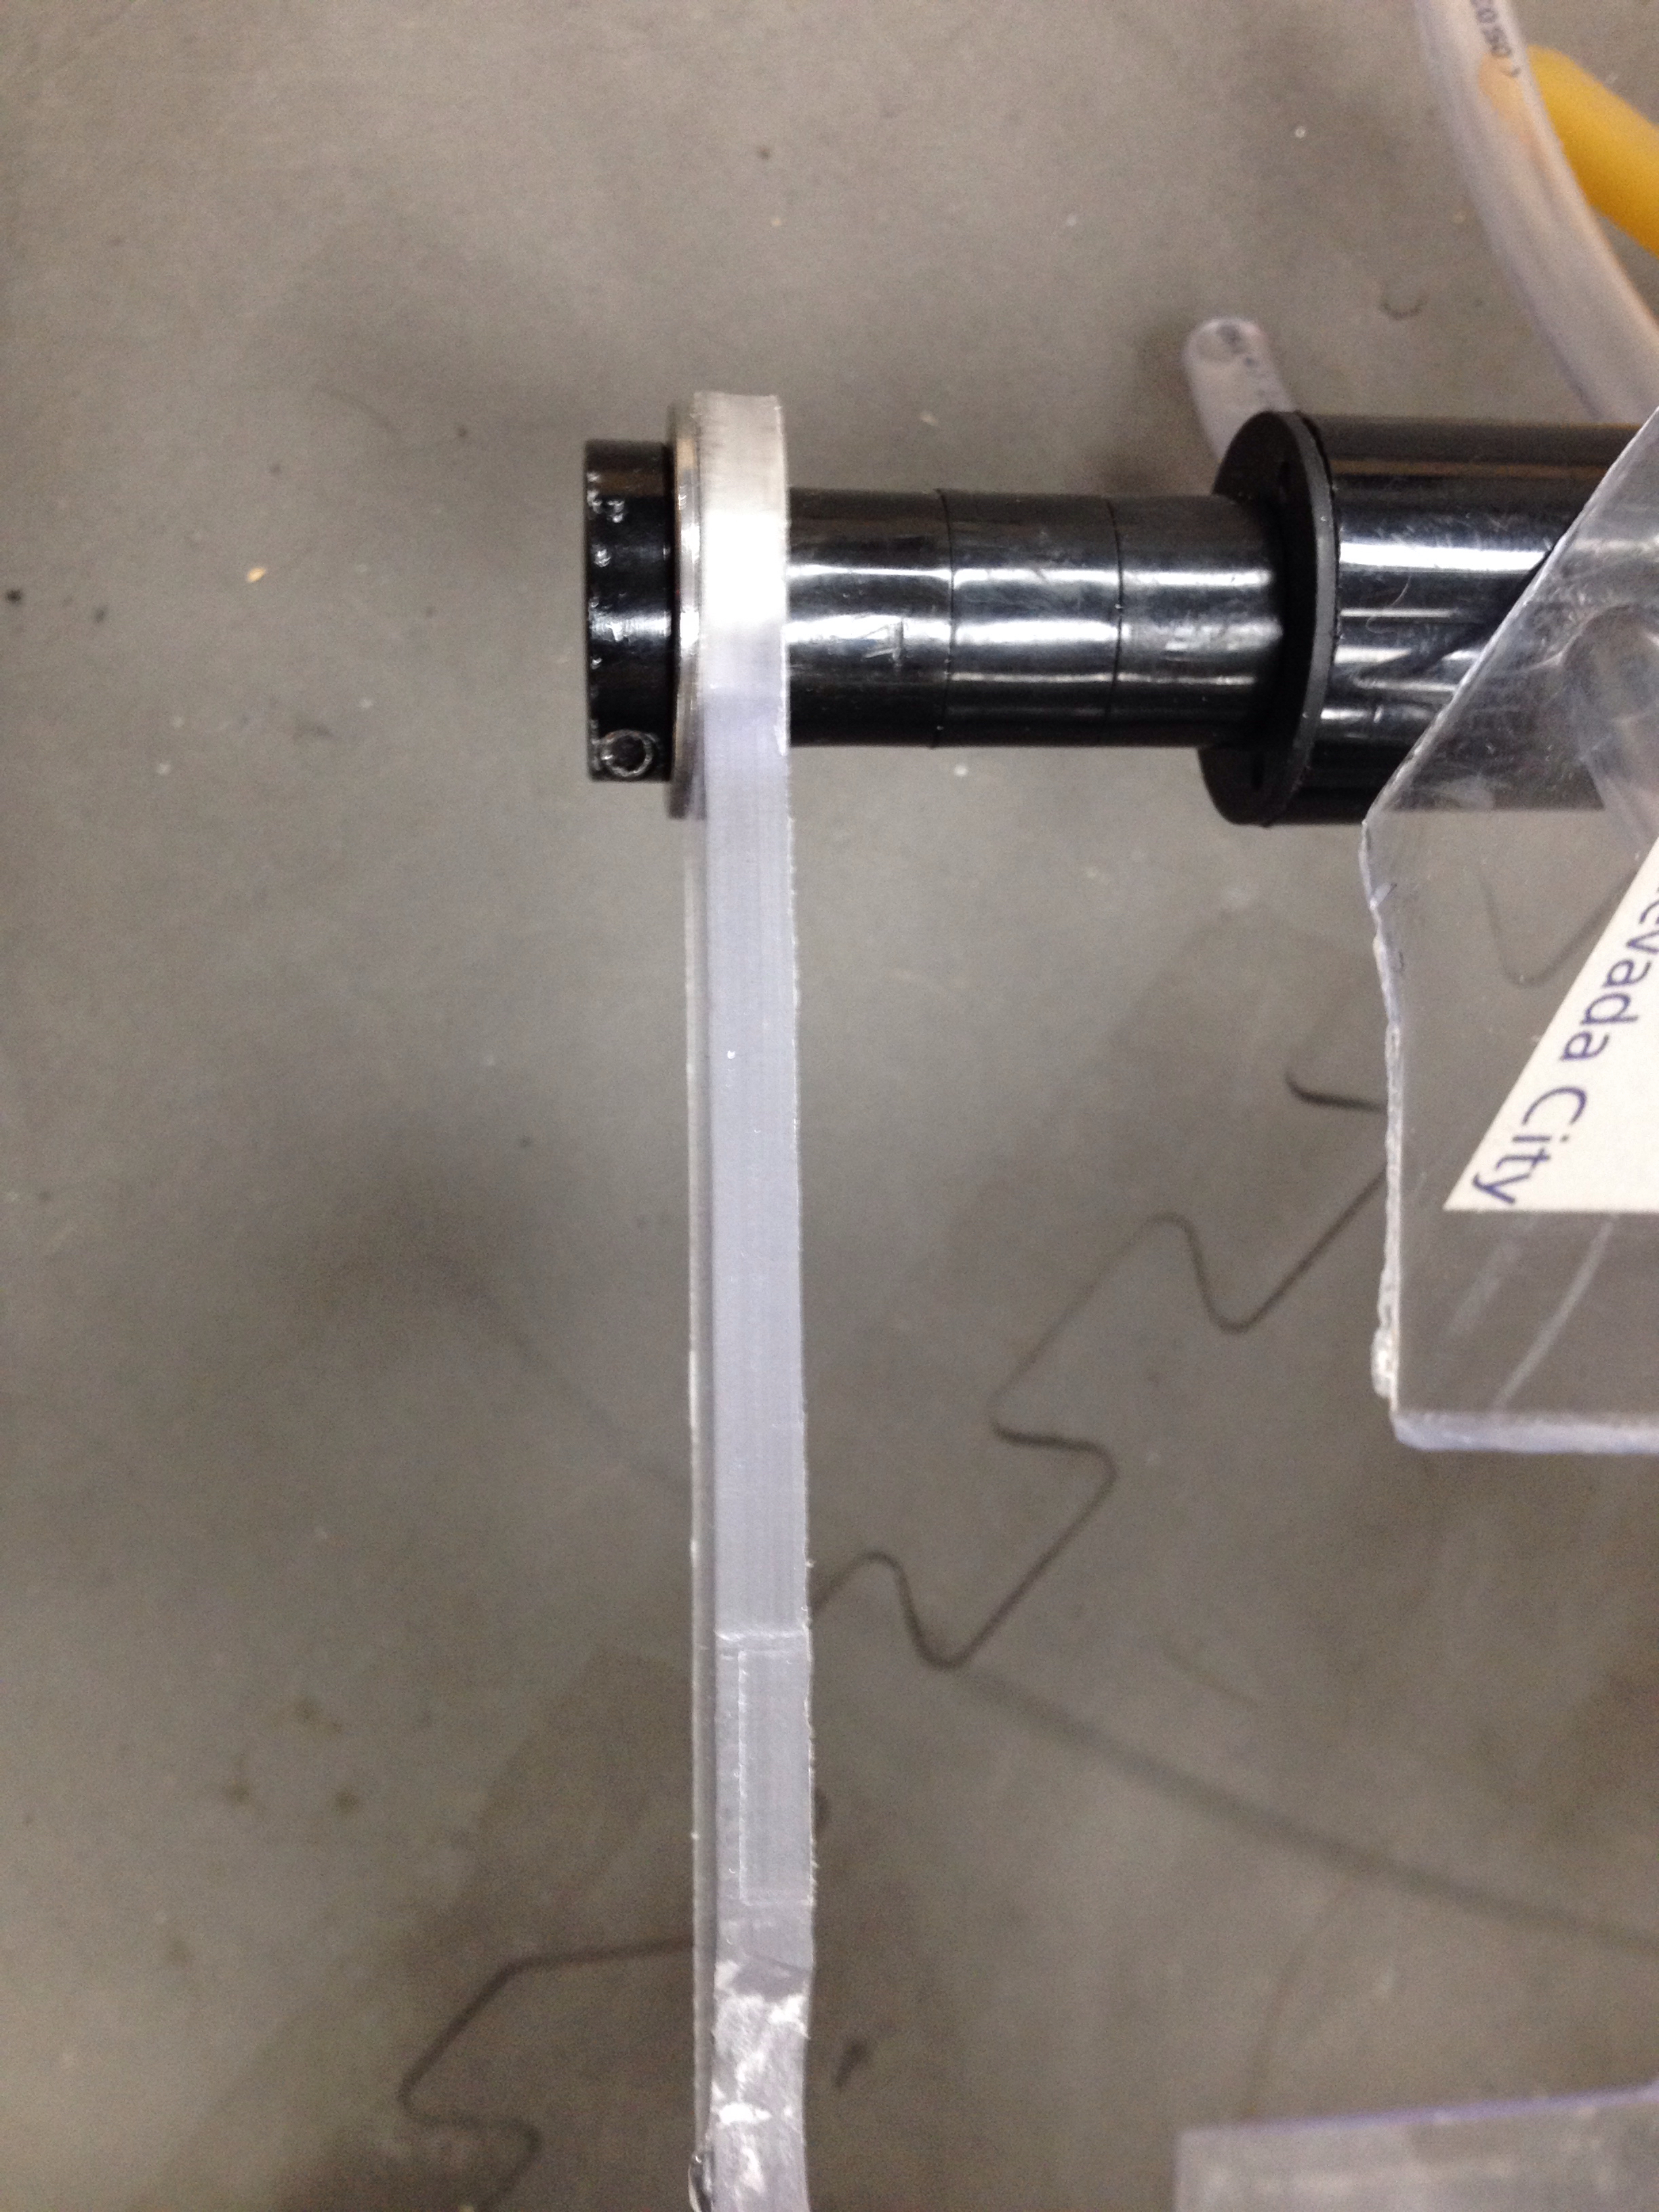
\includegraphics[width= 0.5 \textwidth]{25_02-18/images/Arm.jpg}
    \caption{New Arm}
    \label{fig:arm}
\end{figure}

\begin{figure}
    \centering
    \includegraphics[width= 0.5 \textwidth]{25_02-18/images/phoneMount.png}
    \caption{Phone Case Assembled}
    \label{fig: phone case}
\end{figure}

\subsection{Change lift gear ratio}
%! Find a lift 
After the Napa tournament, the team brainstormed ways to decrease the time it took to score one pair of minerals. 
Because there is such a short distance between the crater and the lander, it takes barely any time to travel between them. 
This meant that the drive team would often be waiting for the lift to reach the top before they could score.
The lift can be made faster by changing the gear ratio of the lift gearbox, however this comes at the expense of torque and could potentially effect the ability of the robot to hang from the lander.
The initial gear ratio had been picked with the conservative safety factors of a 20kg robot under an acceleration of 2g, and was more than enough to lift the robot. 
Kelly re-calculated the ratio with reduced safety factors of a 20kg robot and a 1g acceleration. 
This results in a force of 196 N, and when applied to the 1 in diameter spool this results in 2.483 Nm of torque at the gearbox output shaft.
With the current reduction of 25:1, this resulted in 0.0975 Nm of torque at the motor output shaft
Kelly found that by going to a 18:1 ratio, the torque at the motor output shaft would be .135Nm, which was under the stall torque of .15Nm.
By assuming a new maximum velocity of 20 m/s, instead of the old 14 m/s, and recalculating the motion profiles for the lift, Kelly found that the lift would reach the top in 1.8s, rather than 2.6.
The team ordered a 3:1 and 6:1 stage for the lift gearbox, and swapped it them out for the current reductions.
After the modifications, they verified that the lift indeed did run much faster, while still being able to raise the robot off the ground. 


\subsection{CAD and Fabricate Lift Version 2.0}
%! 
Oren finished the CAD over the weekend to give enough time for the fabricating process, the biggest improvement and change came in the form of the bearing blocks. The blocks were redesigned to be machined out of one bar of aluminum to increase the overall tolerances and strength. Due to the form factor and the assembly of the linear systems inner box frame; it required 2 different styles of blocks (PIC1) (PIC2). Another change that was sought after was the ability to find someone that could weld the inner frame to again strengthen and increase the tolerances. After asking around Oren ended up finding two potential welders, unfortunately the first welder Oren contacted was unable to help due to having a very badly broken leg. But the second contact Chris Kelly (Local Bike Welder) was able to help us, but was only available early next week. Oren then set out to machine all the parts at a sponsoring company GSS, with a team mentor Dan Philips. The machining process took 8 hours over a stint of 2 days to produce all the parts and cut the aluminum tubing, to prep for the welding process next week. 


\begin{figure}
    \centering
    \includegraphics[width= 0.5 \textwidth, angle=270]{25_02-18/images/machining.JPG}
    \caption{Oren machining parts at GSS with Dan}
    \label{fig: oren machining}
\end{figure}



\subsection{New Phone case and  Mounting System}
%!
The old phone case suffered from constant DC's and the Micro USB port on the phones being worn out, leading to more DC's. Ashlin was tasked with making a new phone case that would house the phone permanently and provide a secure connection to the rev hubs. As well as be easily removable from the robot. To do this the case was designed to have a pin system that would allow for removal of the phone in seconds while keeping it secure and positioned correctly for sampling. In Figure \ref{fig: phone case} the top of the case has a bar that is secured with two bolts so that the phone can be removed if needed.

\end{document} 
